\section{The Symbolic World}

Rational thinking, dianoia, does not, and cannot, lead to knowledge of God. Rather, there is a higher form of knowing, traditionally called ``Intuition" which is a direct knowing or realization of metaphysical truths. Since it is based often on the Imagination, discursive reasoning is insufficient. Therefore, Symbols are used in Tradition to convey these higher truths.

The Scholastic principle is that all knowledge begins in the senses. Hence, symbolism is adapted to this need of human nature. Few people are able to begin with pure intellectuality, so the symbols serve as the sensory basis that gives rise to higher levels.

Symbols are both a boon and a bane. For those able to penetrate into the meaning of the symbol, it is a boon. But for the others, it is a bane, because they can only understand the symbols in a literal and material sense. The prime example is alchemy. The alchemical processes have a symbolic meaning which leads to higher states. Understood materially, the ``blowers" attempted to repeat the experiments as if they referred to profane chemistry.

\paragraph{Law of Correspondence}

The multiple states of the being are not isolated from each other. Whatever happens on one plane of existence corresponds to something on another plane. A fortiori, a symbol is not the ``real" meaning of the thing symbolized; instead they are both valid within their own domains. In \emph{Symbolism of the Cross}, \textbf{Rene Guenon} makes this clear:

\begin{quotex}
The fact is that people too often tend to think that if a symbolical meaning is admitted, the literal or historical sense must be rejected; such a view can only result from unawareness of the law of correspondence which is the very foundation of all symbolism. … For this reason the laws of a lower domain can always be taken to symbolize realities of a higher order. 

\end{quotex}
This holds good for historical facts no less than for anything else: they likewise conform to the law of correspondence, and thereby translate higher realities, of which they are a human expression. We would add that it is this that gives to these facts the greater part of their significance.

Hence, the events of sacred history carry a higher meaning without annulling the historical facts. He explains:

\begin{quotex}
This symbolical character, while common to all historical events, is bound to be particularly clear-cut in the case of events connected with what may be called ``sacred history"; thus it is recognizable in a most striking way, in all the circumstances of the life of Christ. If the foregoing has been properly grasped, it will at once be apparent not only that there is no reason for denying the reality of these events and treating them as mere myths, but on the contrary that these events had to be such as they were, and could not have been otherwise. 

\end{quotex}
\paragraph{Documentary}
The temptation when dealing with symbols, myths, legends, and the like is to think in the manner of a televised documentary. A documentary will choose all the variations of the symbols from various and divergent sources, with commentary by various scholars. At the end, one ``knows" a lot of the who, what, where, and men, yet one is no closer to understanding the true meaning of the symbol.

\paragraph{Transmission of Symbols}
Esoteric teachings, when they are made public, are couched in terms of symbols of various types: art, stained glass, icons, legends, myths, fairy tales, and so on. Typically, these symbols are repeated even though they are not fully understood. At the appropriate time, the esoteric meanings of the symbols will be revealed to those ready to understand them.

\begin{wrapfigure}{rt}{.3\textwidth}
 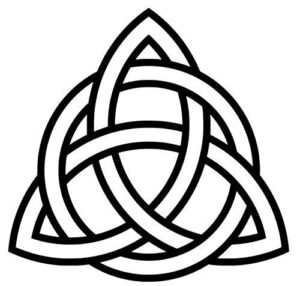
\includegraphics[scale=.3]{a20210403TheSymbolicWorld-img001.jpg}
\end{wrapfigure}

Oftentimes, these legends are repeated and transmitted without being fully understood. Guenon gives as examples, Chrestien de Troyes and Robert de Boron, authors of poetry about the Holy Grail and King Arthur. They are unconscious transmitters, which, however, does not at all diminish their value. Nevertheless, he leaves open the possibility that they were aware of what they were transmitting.

On the other hand, Guenon mentions Dante and the authors of the Romance of the Rose as conscious transmitters of esoteric doctrines.

\paragraph{Hiding the Bone}
The real meaning of an esoteric text is often hidden and ``sometimes they hide it too well," as Guenon says. He lists various techniques to hide the true meaning from those not ready for it:

\begin{quotex}
There is a mixture of insignificant and incoherent elements … obscurities and even contradictions may be perfectly intentional and seemingly pointless details may have the express purpose of leading astray the attention of the profane, just as a symbol can be hidden in a more or less complicated motif of ornamentation. 

\end{quotex}
In other esoteric writings, those of Rabelais and Boccacio, for example, humour and even sexual inuendo may be used to hide the true meaning.

\paragraph{Multivocal Meanings}
Symbols seldom have a univocal meaning, as there may be multiple interpretations. Guenon elaborates:

\begin{quotex}
A consequence of this law of correspondence is the plurality of meanings contained in every symbol. Anything and everything can be regarded as representing not only the metaphysical principles, but also realities of all orders higher than its own … These multiple and hierarchically superimposed symbolical meanings are not in any way mutually exclusive. 

\end{quotex}
For the most part, we are interested in the metaphysical sense of the symbol, since it is the first and most important of all. That is because it is principial, i.e., based on metaphysical principles.



\flrightit{Posted on 2021-04-03 by Cologero }

\begin{center}* * *\end{center}

\begin{footnotesize}\begin{sffamily}



\texttt{Michael M on 2021-04-03 at 13:20 said: }

``For the most part, we are interested in the metaphysical sense of the symbol, since it is the first and most important of all. That is because it is principial, i.e., based on metaphysical principles."

This is a representation of Being and its descent, everything really, it is a law of all. From the first principal that the symbol can point to, certain manifestations come out of such a process and then are represented in the symbol. Descending further man gazes upon symbols and gives it existence in Creation through his consciousness, his participation as a form of manifestation and action. Thus the whole great chain of Being is not only manifested, it is also thought of and adored and created perpetually.

``the Divine Artificer still longed for some creature which might comprehend the meaning of so vast an achievement, which might be moved with love at its beauty and smitten with awe at its grandeur."

So while the horizontal and vertical can seem at odds, especially with how the World is today, it is more accurate that Man chooses to descend, as much as he chooses to ascend. Let myself and let us all not throw away the myths and symbols, instead take them in a chew on them all the way to the marrow. The junk of modernity progresses only to death, instead of the bread of life.

``I will not walk with your progressive apes,

erect and sapient. Before them gapes

the dark abyss to which their progress tends

if by God's mercy progress ever ends,

and does not ceaselessly revolve the same

unfruitful course with changing of a name.

I will not treat your dusty path and flat,

denoting this and that by this and that,

your world immutable wherein no part

the little maker has with maker's art.

I bow not yet before the Iron Crown,

nor cast my own small golden sceptre down."


\end{sffamily}\end{footnotesize}
